\def\inc{inc2-5-mem}

\titreA {Gestion de la mémoire}

%%%%%%%%%%%%%%%%%%%%%%%%%%%%%%%%%%%%%%%%%%%%%%%%%%%%%%%%%%%%%%%%%%%%%%%%%%%%%%
% Introduction
%%%%%%%%%%%%%%%%%%%%%%%%%%%%%%%%%%%%%%%%%%%%%%%%%%%%%%%%%%%%%%%%%%%%%%%%%%%%%%

\titreB {Introduction}

\begin {frame} {Introduction}
    Comment :
    \begin {enumerate}
	\item faire cohabiter plusieurs processus en mémoire ?
	    \begin {itemize}
		\item ... tout en garantissant la sécurité des données
	    \end {itemize}
	\item attribuer de la mémoire à tous les processus ?
	    \begin {itemize}
		\item pas au même instant \implique swap
	    \end {itemize}
	\item exécuter des processus plus grands que la mémoire ?
	    \begin {itemize}
		\item mémoire virtuelle et pagination
	    \end {itemize}
    \end {enumerate}

    \vspace* {3mm}

    Rappel : mécanisme matériel indispensable
    \begin {itemize}
	\item unité de gestion de mémoire
	\item memory management unit (MMU)
    \end {itemize}
\end {frame}

%%%%%%%%%%%%%%%%%%%%%%%%%%%%%%%%%%%%%%%%%%%%%%%%%%%%%%%%%%%%%%%%%%%%%%%%%%%%%%
% Traduction d'adresses
%%%%%%%%%%%%%%%%%%%%%%%%%%%%%%%%%%%%%%%%%%%%%%%%%%%%%%%%%%%%%%%%%%%%%%%%%%%%%%

\titreB {Traduction d'adresses}

\begin {frame} {Traduction d'adresses}

    Rappel : espace d'adressage logique d'un processus

    \vspace* {2mm}

    \begin {minipage} {.55\linewidth}
	Chaque processus dispose~:
	\begin {itemize}
	    \item du segment «~\emph {text}~» \\
		(non modifiable)
	    \item du segment «~\emph {data}~» \\
		(extensible via \texttt {malloc})
	    \item du segment «~\emph {stack}~» \\
		(extensible automatiquement)
	    \item et éventuellement d'autres
		segments (bibliothèques dynamiques...)
	\end {itemize}

    \end {minipage}
    \hfill
    \begin {minipage} {.43\linewidth}
	\begin {center}
	\includegraphics [width=.7\linewidth] {\inc/ps-mem}
	\end {center}
    \end {minipage}
\end {frame}

\begin {frame} {Traduction d'adresses}
    Chaque processus a son propre espace d'adressage~:

    \begin {minipage} {.58\linewidth}

	Les programmes utilisent des adresses \textit {relatives} à
	l'espace d'adressage du processus.

	\vspace* {3mm}

	Exemple~: un programme utilise la case mémoire d'adresse
	1000. Si deux processus exécutent ce programme, chacun doit
	avoir sa propre case d'adresse 1000. Ces deux cases ont
	une adresse réelle différente en mémoire.

    \end {minipage}
    \hfill
    \begin {minipage} {.40\linewidth}
	\begin {center}
	    \includegraphics [width=.9\linewidth] {\inc/trans-adr}
	\end {center}
    \end {minipage}
\end {frame}

\begin {frame} {Traduction d'adresses -- MMU simple}

    Unité de gestion mémoire (MMU)~:
    \begin {center}
	\includegraphics [width=.7\linewidth] {\inc/mmu-princ}
    \end {center}

    \begin {itemize}
	\item MMU : composant matériel
	\item CPU présente une adresse logique sur le bus d'adresses
	\item si adresse $\geq$ limite, alors exception
	\item si adresse < limite, alors MMU calcule l'adresse physique \\
	    (adresse physique = adresse logique + limite)
    \end {itemize}
\end {frame}

\begin {frame} {Traduction d'adresses -- MMU simple}
    Cette MMU est irréaliste~: trop simple pour les cas réels

    \begin {itemize}
	\item pas de prise en compte de l'adresse 0
	\item les processus ont des «~trous~» dans leur espace
	    d'adressage \\
	    (ex~: espace entre segment «~data~» et «~stack~»)
	\item les segments d'un processus ne sont pas forcément contigüs
	    en mémoire physique
	\item pas de possibilité de partager un segment \\
	    (ex~: partage du segment «~text~» entre processus)
    \end {itemize}

    \implique mais elle est pédagogique !

\end {frame}

\begin {frame} {Traduction d'adresses -- MMU simple}

    Retour sur la commutation de processus

    \vspace* {1mm}

    Avec notre MMU simpliste, il suffit~:

    \vspace* {1mm}

    \begin {minipage} {.45\linewidth}

	\begin {itemize}
	    \item de considérer qu'il n'y a pas de traduction
		d'adresse lorsque le CPU est en mode «~système~»

	    \item d'intégrer les deux registres «~limite~» et «~base~»
		lors de la sauvegarde et de la restauration des
		registres

	    \item de vider le cache

	\end {itemize}

    \end {minipage}
    \hfill
    \begin {minipage} {.53\linewidth}
	\includegraphics [width=\linewidth] {\inc/ps-commut}
	\\
	\centerline {\tiny (Même dessin que précédemment)}
    \end {minipage}
\end {frame}

\begin {frame} {Traduction d'adresses -- HP 9000 IPC}

    Unité de gestion mémoire du HP 9000-IPC~:

    \begin {minipage} {.69\linewidth}
	\begin {center}
	    \includegraphics [width=.8\linewidth] {\inc/mmu-ipc}
	\end {center}
    \end {minipage}
    \hfill
    \begin {minipage} {.30\linewidth}
	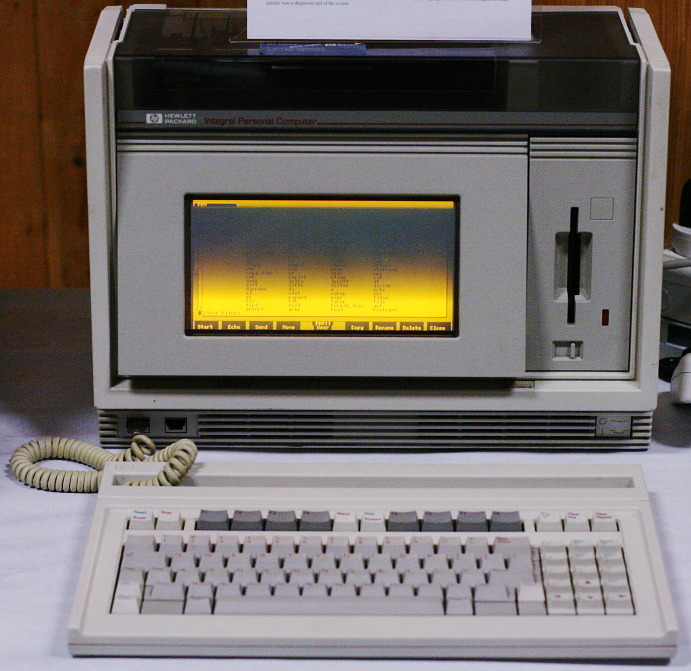
\includegraphics [width=\linewidth] {\inc/hp-ipc}
	\\
	\creditphoto {Wolfgang Steif} {\ccby}
    \end {minipage}

    \begin {itemize}
	\item MMU «~câblée~»
	\item type d'accès mémoire (U/S, D/P) \implique registre consulté
	\item additionneur seul \implique pas de vérification de limite \\
	    (machine mono-utilisateur)
    \end {itemize}

\end {frame}

\begin {frame} {Traduction d'adresses -- PDP 11/45}

    Principe de l'unité de gestion mémoire du PDP 11/45~:

    \begin {minipage} {.59\linewidth}
	\begin {center}
	    \includegraphics [width=.8\linewidth] {\inc/mmu-pdp11a}
	\end {center}
    \end {minipage}
    \hfill
    \begin {minipage} {.39\linewidth}
	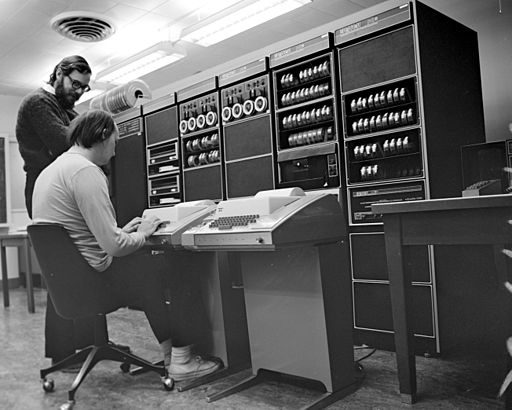
\includegraphics [width=\linewidth] {\inc/pdp11}
	\\
	\creditphoto {Dennis Ritchie} {\ccbysa}
    \end {minipage}

    \vspace* {3mm}

    \begin {itemize}
	\item espace d'adressage d'un processus découpé en 8 segments
	\item mémoire physique découpée en blocs de $2^6$ octets
	\item chaque segment est traduit par un registre de la MMU

    \end {itemize}

\end {frame}

\begin {frame} {Traduction d'adresses -- PDP 11/45}

    Traduction d'adresse sur le PDP 11/45~:

    \begin {center}
	\includegraphics [width=.45\linewidth] {\inc/mmu-pdp11b}
    \end {center}

    \begin {itemize}
	\item mémoire physique découpée en blocs de $2^6$ octets
	\item limite d'un segment : sur 7 bits
	\item jusqu'à 8 segments entre 1 et 2$^7$ blocs (64 à
	    8192 octets)

    \end {itemize}
\end {frame}

\begin {frame} {Placement des processus en mémoire}
    Où placer un processus en mémoire ?

    \begin {itemize}
	\item Le noyau gère une « carte » des emplacements en mémoire
	    \begin {itemize}
		\item besoin de mémoire : trouver une entrée dans la « carte »
	    \end {itemize}
	\item Algorithmes classiques
	    \begin {itemize}
		\item \textit {first fit} : le premier
		    emplacement suffisamment grand
		    \begin {itemize}
			\item simple ! utilisé sur Unix originel
		    \end {itemize}
		\item \textit {best fit} : le plus petit
		    emplacement suffisamment grand
		\item \textit {worst fit} : le plus grand
		    emplacement
		    \begin {itemize}
			\item le moins bon des trois en terme
			    d'utilisation de la mémoire
		    \end {itemize}
	    \end {itemize}
	\item Attention à la « fragmentation » de la mémoire
	    \begin {itemize}
		\item compactage de la mémoire
		    \begin {itemize}
			\item pas sur Unix originel
		    \end {itemize}
	    \end {itemize}
    \end {itemize}
\end {frame}

\begin {frame} {Partage de mémoire}
    MMU \implique possibilité de partager des portions de mémoire :

    \begin {itemize}
	\item segment «~\textit {text}~» non modifiable :
	    \begin {itemize}
		\item si plusieurs processus utilisent le même programme
		    \\
		    alors partage du segment «~text~»

		    \begin {itemize}
			\item exemple : après \code {fork}, le segment
			    «~\textit {text}~» n'est pas dupliqué
			\item partage « invisible » pour les processus
			\item le noyau mémorise la référence au
			    fichier exécutable (i.e. l'inode) de
			    chaque processus
		    \end {itemize}
		\end {itemize}

	\item partage de mémoire entre processus
	    \begin {itemize}
		\item plein de problèmes intéressants...
		\item ... voir cours de systèmes concurrents, semestre 5
	    \end {itemize}
    \end {itemize}
\end {frame}


%%%%%%%%%%%%%%%%%%%%%%%%%%%%%%%%%%%%%%%%%%%%%%%%%%%%%%%%%%%%%%%%%%%%%%%%%%%%%%
% Swap
%%%%%%%%%%%%%%%%%%%%%%%%%%%%%%%%%%%%%%%%%%%%%%%%%%%%%%%%%%%%%%%%%%%%%%%%%%%%%%

\titreB {Swap}

\begin {frame} {Swap}
    Que se passe-t'il si toute la mémoire est occupée et qu'il y a un
    besoin de mémoire supplémentaire ?
    \begin {itemize}
	\item un nouveau processus est créé, ou
	\item un processus existant demande un agrandissement
	    \begin {itemize}
		\item utilisation de \code {malloc} (primitive \code {sbrk})
		\item utilisation de la pile
	    \end {itemize}
    \end {itemize}

    \vspace* {3mm}
    
    Swap :

    \begin {itemize}
	\item un ou plusieurs processus sont choisis pour être
	    «~évincés~» (\textit {swap-out}) de la mémoire...

	    \begin {itemize}
		\item ... et recopiés vers une partie du disque
		    (espace de swap)
	    \end {itemize}

	\item la mémoire libérée est réutilisable

	\item il faudra ultérieurement ramener (\textit {swap-in})
	    ces processus en mémoire

	\item si plus assez de place dans l'espace de swap \implique kill !

    \end {itemize}
\end {frame}

\begin {frame} {Swap}
    Problèmes :
    \begin {enumerate}
	\item comment gérer l'espace de swap ?
	    \begin {itemize}
		\item système comparable à la gestion de l'espace mémoire
		\item \implique « carte » de l'espace de swap
	    \end {itemize}
	\item quels processus choisir ?
	    \begin {itemize}
		\item pour évincer ?
		\item pour ramener ?
		\item en évitant le «~\textit {trashing}~» (écroulement) ?
	    \end {itemize}
    \end {enumerate}
\end {frame}

\begin {frame} {Évincement -- Choix}
    Quel processus évincer ? Paramètres du choix :
    \begin {itemize}
	\item temps de résidence (en mémoire, ou sur le swap)
	\item état (prêt, ou en attente de ressource)
    \end {itemize}
\end {frame}

\begin {frame} {Évincement -- Choix}
    Exemple : Unix (originel)
    \begin {itemize}
	\item évincement
	    \begin {itemize}
		\item tant que le besoin en mémoire n'est pas satisfait
		    \begin {itemize}
			\item prendre le plus grand parmi les processus
			    en attente
			\item sinon, prendre le processus prêt
			    résident en mémoire depuis la plus longue
			    durée
		    \end {itemize}
	    \end {itemize}
	\item ramener en mémoire
	    \begin {itemize}
		\item parmi les processus prêts, choisir celui qui est
		    sur le swap depuis la plus longue durée
	    \end {itemize}
	\item prévenir le « \textit {trashing}~»
	    \begin {itemize}
		\item utiliser des seuils
		    \begin {itemize}
			\item ne pas évincer les processus prêts s'ils
			    sont en mémoire depuis moins de 2 secondes
			\item ne pas ramener les processus en mémoire
			    s'ils sont sur le swap depuis moins de
			    3 secondes
		    \end {itemize}
	    \end {itemize}
    \end {itemize}
\end {frame}

%%%%%%%%%%%%%%%%%%%%%%%%%%%%%%%%%%%%%%%%%%%%%%%%%%%%%%%%%%%%%%%%%%%%%%%%%%%%%%
% Mémoire virtuelle et pagination
%%%%%%%%%%%%%%%%%%%%%%%%%%%%%%%%%%%%%%%%%%%%%%%%%%%%%%%%%%%%%%%%%%%%%%%%%%%%%%

\titreB {Mémoire virtuelle et pagination}

\begin {frame} {Mémoire virtuelle}
    Jusqu'ici, traduction mémoire «~simple~»

    \begin {itemize}
	\item mémoire d'un processus : divisée en
	    $p$ blocs de $2^k$ octets

	    Sur PDP 11/45~: $p=2^3 = 8$, $k=13$ \implique $2^k = 8192$ octets

	\item adapté pour les 3 segments d'un processus \\
	    et peut-être d'autres segments supplémentaires
	    (bibliothèques dynamiques, mémoire partagée, etc.)

	\item pour que le processus soit mis sur le processeur,
	    il faut que tout son espace d'adressage soit en mémoire
    \end {itemize}
\end {frame}

\begin {frame} {Mémoire virtuelle}

    Besoins nouveaux~:
    \begin {itemize}
	\item exécuter des programmes de taille supérieure à la
	    mémoire physique

	\item rationaliser l'utilisation de la mémoire \\
	    un processus n'a pas besoin de tout son espace d'adressage
	    pendant toute sa durée de vie

	    Exemple : code d'initialisation parcouru une seule
	    fois
    \end {itemize}

    \vspace* {3mm}

    \implique Mémoire virtuelle (pagination)

\end {frame}

\begin {frame} {Mémoire virtuelle}

    Principes~:

    \begin {itemize}
	\item l'espace mémoire est découpé en \textbf {pages} de taille $2^n$ \\
	    Ex~: $n = 12$ \implique $2^n = 4096$ octets (cas le plus courant) \\
	    Ex~: $n = 22$ \implique $2^n = 4$ Mo (\emph {superpages}
		sur x86)

	\item chaque page peut être chargée en mémoire ou non

	\item la MMU gère une «~table des pages~» par processus

	\item «~défaut de page~» : la MMU génère une exception \\
	    \implique le noyau traite l'exception
	
	\item lorsque le noyau aura chargé la page en mémoire et
	    positionné la table des pages, le processeur pourra à
	    nouveau tenter l'exécution de l'instruction «~fautive~»
	    \\
	    \implique les instructions sont «~redémarrables~»

    \end {itemize}

\end {frame}

\begin {frame} {Mémoire virtuelle}

    Unité de gestion mémoire du i386~:

    \begin {center}
	\includegraphics [width=\linewidth] {\inc/mmu-i386}
    \end {center}
\end {frame}

\begin {frame} {Mémoire virtuelle}

    Exemple du i386~:

    \begin {itemize}
	\item segmentation : poids du passé, on oublie...
	\item adresse après segmentation sur 32 bits
	\item la table «~page directory~» est~:
	    \begin {itemize}
		\item référencée par le registre CR3 du processeur
		\item indexée par les 12 bits de poids fort de l'adresse
	    \end {itemize}
	\item chaque table des pages est~:
	    \begin {itemize}
		\item référencée par l'entrée dans «~page directory~»
		\item indexée par les 12 bits de poids milieu de l'adresse
	    \end {itemize}
	\item l'adresse physique est constituée~:
	    \begin {itemize}
		\item de l'adresse de la page trouvée dans la table des page
		\item de l'offset dans la page récupéré de l'adresse originale
	    \end {itemize}

    \end {itemize}

\end {frame}

\begin {frame} {Mémoire virtuelle}
    Les tables des pages résident en mémoire~:

    \begin {itemize}
	\item commutation de processus \implique changer l'adresse de la
	    table des pages
	    \\
	    (registre CR3 sur x86)

	\item les tables de pages peuvent être swappées sur le disque

	\item la traduction d'une adresse peut elle-même conduire
	    à un défaut de page

	\item traduction lente, même sans défaut de page \\
    \end {itemize}

    Optimisation des traductions~:
    \begin {itemize}
	\item TLB (\emph {Translation Lookaside Buffer\/}) \\
	    \implique cache des dernières traductions d'adresse \\

    \end {itemize}

\end {frame}

\begin {frame} {Mémoire virtuelle}

    Exemple pour Pentium III (x86)~: TLB «~\emph {4-way set-associative}~»

    \begin {center}
	\includegraphics [width=.9\linewidth] {\inc/mmu-tlb386}
    \end {center}

    {\footnotesize Ne pas oublier de vider le TLB lors de la commutation
    de processus...}
\end {frame}

\begin {frame} {Flags de page}
    Plusieurs bits sont associés à chaque page dans la table des pages :

    \ctableau {\fC} {|c|p{.75\linewidth}|} {
	\rca \textbf {Bit} &
	    \multicolumn {1} {c|} {\textbf {Comportement de la MMU}}
	    \\
	\rcb \textit {valid} &
	    générer une exception si le processeur tente
	    d'accéder à une page n'ayant pas ce bit
	    \\
	\rca \textit {read-only} &
	    générer une exception si le processeur tente
	    de modifier une page ayant ce bit
	    \\
	\rcb \textit {no-execute} &
	    générer une exception si le processeur tente
	    d'exécuter une instruction d'une page ayant ce bit
	    \\
	\rca \textit {supervisor} &
	    générer une exception si le processeur tente d'accéder
	    à la page alors qu'il est en mode non privilégié
	    \\
	\rcb \textit {accessed} &
	    positionner ce bit en cas d'accès
	    (lecture, écriture ou exécution) à la page
	    \\
	\rca \textit {dirty} &
	    positionner ce bit en cas d'accès en écriture à
	    la page
	    \\
    }

    Note : certaines MMU ne gèrent pas tous ces bits
\end {frame}

\begin {frame} {Flags de page -- Bit « valid »}
    Utilisations du bit « \textit {valid} » : 

    \begin {itemize}
	\item \textit {swap} :
	    \begin {itemize}
		\item les pages individuelles peuvent être évincées
	    \end {itemize}
	\item \textit {load-on-demand} :
	    \begin {itemize}
		\item \code {exec} : chargement à partir de l'exécutable
		    \implique illusion
		\item en réalité : \code {exec} marque toutes les pages
		    comme invalides
		    \begin {itemize}
			\item tentative d'exécution de la première instruction
			    \\
			    \implique défaut de page \\
			    \implique chargement de la première page du code
			\item tentative de lecture/modification de variable
			    \\
			    \implique défaut de page
			    \\
			    \implique chargement de la page correspondante
			    des données

			\item etc.
		    \end {itemize}
		\item le noyau conserve la source de chaque page du processus :
		    \begin {itemize}
			\item fichier exécutable (code, données initialisées)
			\item 0 (données non initialisées, pile)
			\item espace de swap (page modifiée et swappée)
		    \end {itemize}
	    \end {itemize}
    \end {itemize}
\end {frame}

\begin {frame} {Flags de page -- Bit « read-only »}
    Utilisations du bit « \textit {read-only} » : 
    \begin {itemize}
	\item pour les pages naturellement en lecture seule
	    \begin {itemize}
		\item exemple : segment « \textit {text} »
		\item exemple : segment « \textit {vdso} » sur Linux
		    \begin {itemize}
			\item le noyau met à disposition des processus
			    une page en lecture seule pour «~exporter~»
			    certaines données (pid, heure courante, etc.)
			    pour accélérer certaines primitives systèmes
			    (\code {getpid}, \code {gettimeofday}, etc.)
			\item pas de passage en mode privilégié
		    \end {itemize}
	    \end {itemize}
	\item \textit {copy-on-write} :
	    \begin {itemize}
		\item \code {fork} : duplique la mémoire \implique illusion
		    \begin {itemize}
			\item les pages modifiables sont marquées «~read-only~»
			    dans les deux processus
			\item si un processus tente d'écrire \implique exception
			\item le noyau duplique alors la page et la remet
			    en «~lecture/écriture~» pour les deux processus
		    \end {itemize}
		\item réduit drastiquement le coût de \code {fork} !
	    \end {itemize}
    \end {itemize}
\end {frame}

\begin {frame} {Flags de page -- Bit « no-execute »}
    Utilisations du bit « \textit {no-execute} » : 
    \begin {itemize}
	\item bit récent, pour réduire les problèmes de sécurité
	\begin {itemize}
	    \item problème classique de «~débordement de tampon~»
	    \item injection de code exécutable par un pirate
		\begin {itemize}
		    \item typiquement dans les données ou la pile
		    \item page marquée «~no-execute~» \implique
			injection inopérante
		\end {itemize}
	\end {itemize}
    \end {itemize}
\end {frame}

\begin {frame} {Flags de page -- Bit « dirty »}
    Utilisations du bit « \textit {dirty} » : 
    \begin {itemize}
	\item pour savoir si une page doit être swappée ou non
	    \begin {itemize}
		\item lorsque le noyau recherche de la place en mémoire,
		    il doit supprimer des pages
		\item si la page a été modifiée, elle doit être
		    sauvegardée dans l'espace de swap
		\item si la page n'est pas modifiée, elle pourra être
		    rechargée à partir de sa source :
		    \begin {itemize}
			\item fichier exécutable (code, données initialisées)
			\item 0 (données non initialisées, pile)
			\item espace de swap (page modifiée et swappée)
		    \end {itemize}
		    \implique économie d'une recopie dans l'espace de swap
	    \end {itemize}
    \end {itemize}
\end {frame}

\begin {frame} {Flags de page -- Bit « accessed »}
    Utilisations du bit « \textit {accessed} » : 
    \begin {itemize}
	\item détermination du «~\textit {working set}~» des processus
	    \begin {itemize}
		\item localité temporelle : si une page a été accédée
		    récemment, il est probable qu'elle sera à nouveau
		    accédée prochainement
		\item permet de déterminer quelles pages il faut swapper
		\item mécanisme périodique :
		    \begin {itemize}
			\item le noyau remet toutes les pages à «~non
			    accédée~»
			\item les processus s'exécutent \implique la
			    MMU marque toutes les pages accédées
			\item au bout d'un certain temps, toutes les pages
			    encore marquées «~non accédées~» peuvent être
			    évincées s'il y a un besoin de mémoire
		    \end {itemize}
	    \end {itemize}
    \end {itemize}
\end {frame}

\begin {frame} {Flags de page -- Bits manquants}
    Certaines MMU n'ont pas tous les bits \implique émulation

    \vspace* {3mm}

    Exemples :

    \begin {itemize}
	\item pas de bit «~\textit {accessed}~»
	    \begin {itemize}
		\item pour déterminer le «~\textit {working set}~» :
		    \begin {itemize}
			\item rendre toutes les pages invalides
			\item dès qu'il y a un défaut de page, et si
			    la page est réellement présente, le noyau
			    peut la marquer «~\textit {accessed}~»
		    \end {itemize}
	    \end {itemize}
	\item pas de bit «~\textit {read-only}~»
	    \begin {itemize}
		\item pour réaliser le «~\textit {copy-on-write}~» :
		    \begin {itemize}
			\item rendre toutes les pages invalides
			\item dès qu'il y a un défaut de page, si
			    la page est présente et qu'elle résulte
			    d'un partage, le noyau peut réaliser le
			    «~\textit {copy-on-write}~»
		    \end {itemize}
	    \end {itemize}
    \end {itemize}
\end {frame}
